% appendix
\newlength{\chaptertopskip}
\setlength{\chaptertopskip}{0pt}
\makeatletter
\xpatchcmd{\@makechapterhead}{\vspace*{50\p@}}{\vspace*{\chaptertopskip}}{\typeout{Success}}{\typeout{Failure!!!}}
\makeatother

\chapter{EV Simulink model - figures}
\label{appendix}



\rotatebox{90}{
\begin{minipage}{0.85\textheight}
    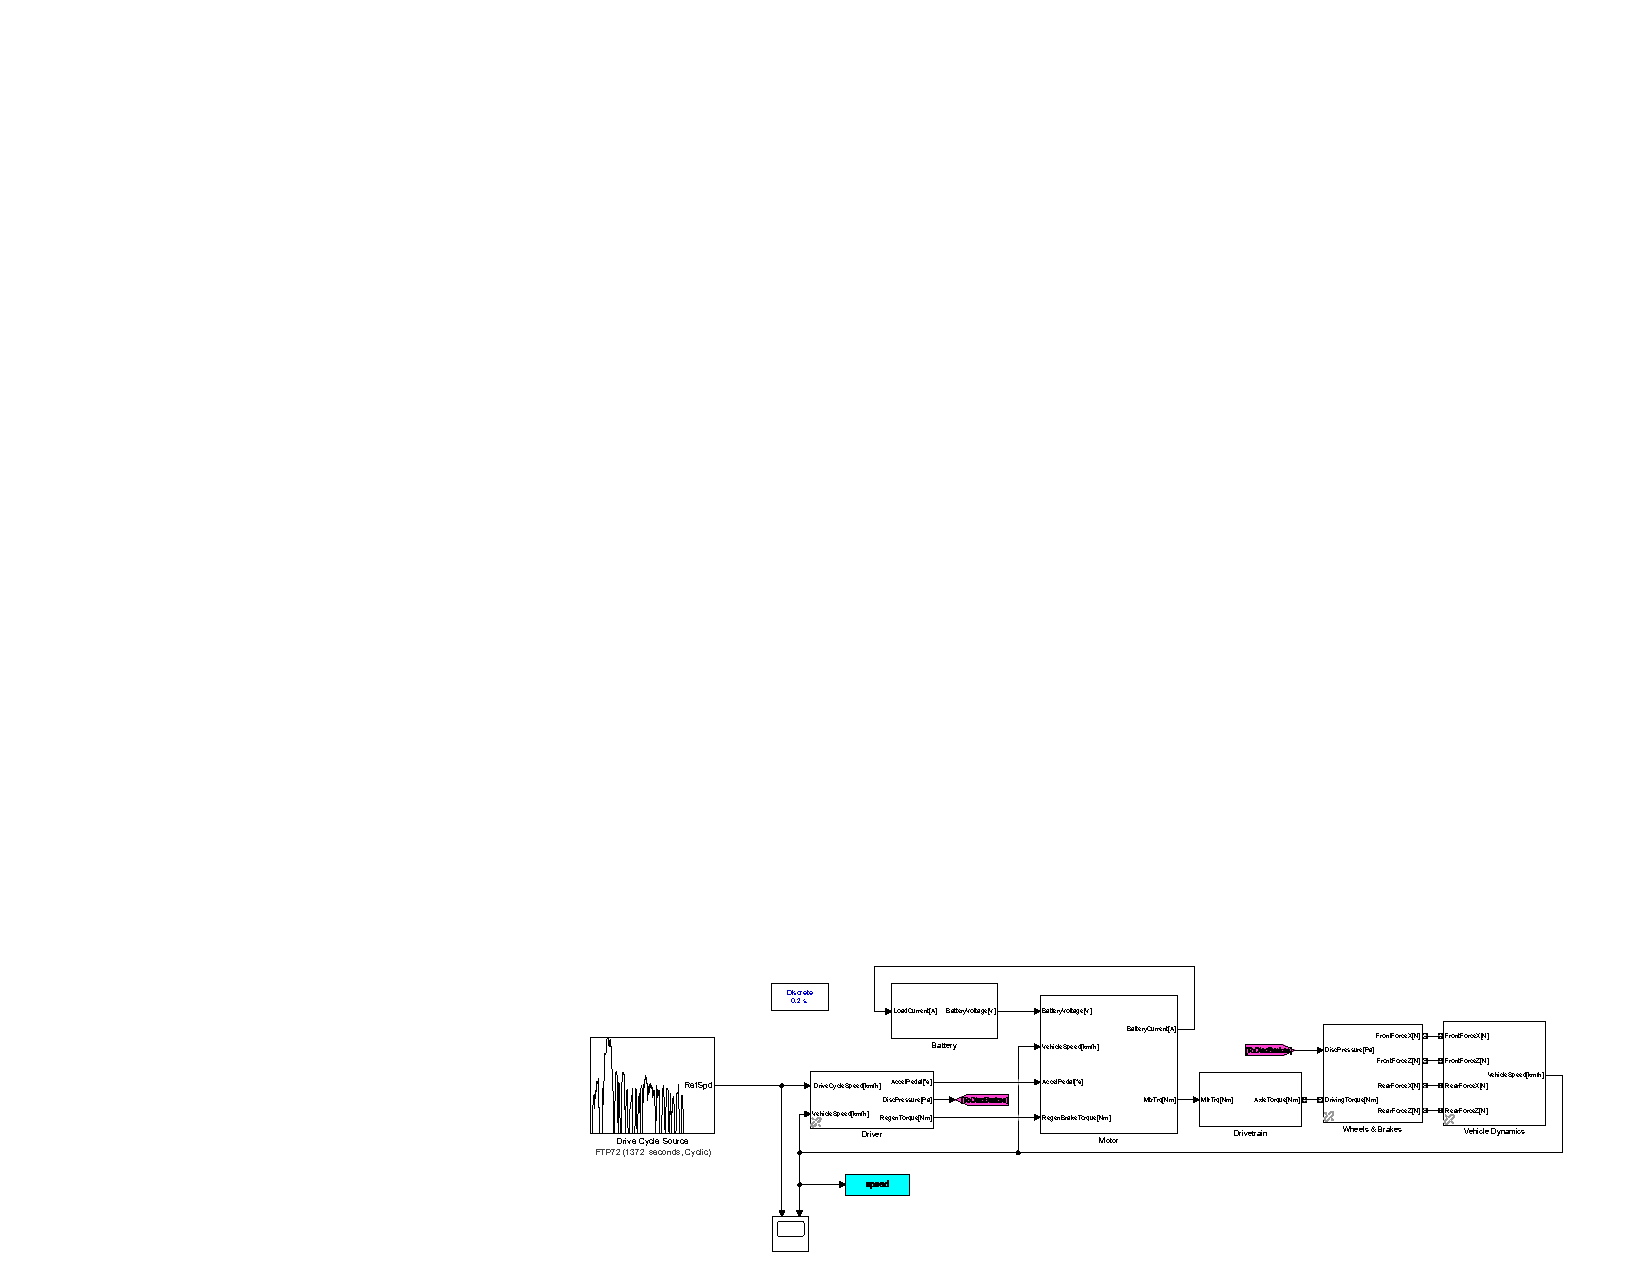
\includegraphics[width=\textwidth]{images/electricvehicle}
    \captionof{figure}{Simulink EV model}
    \label{fig:ev_model}
\end{minipage}
}
\hspace{3cm}
\rotatebox{90}{
\begin{minipage}{0.85\textheight}
    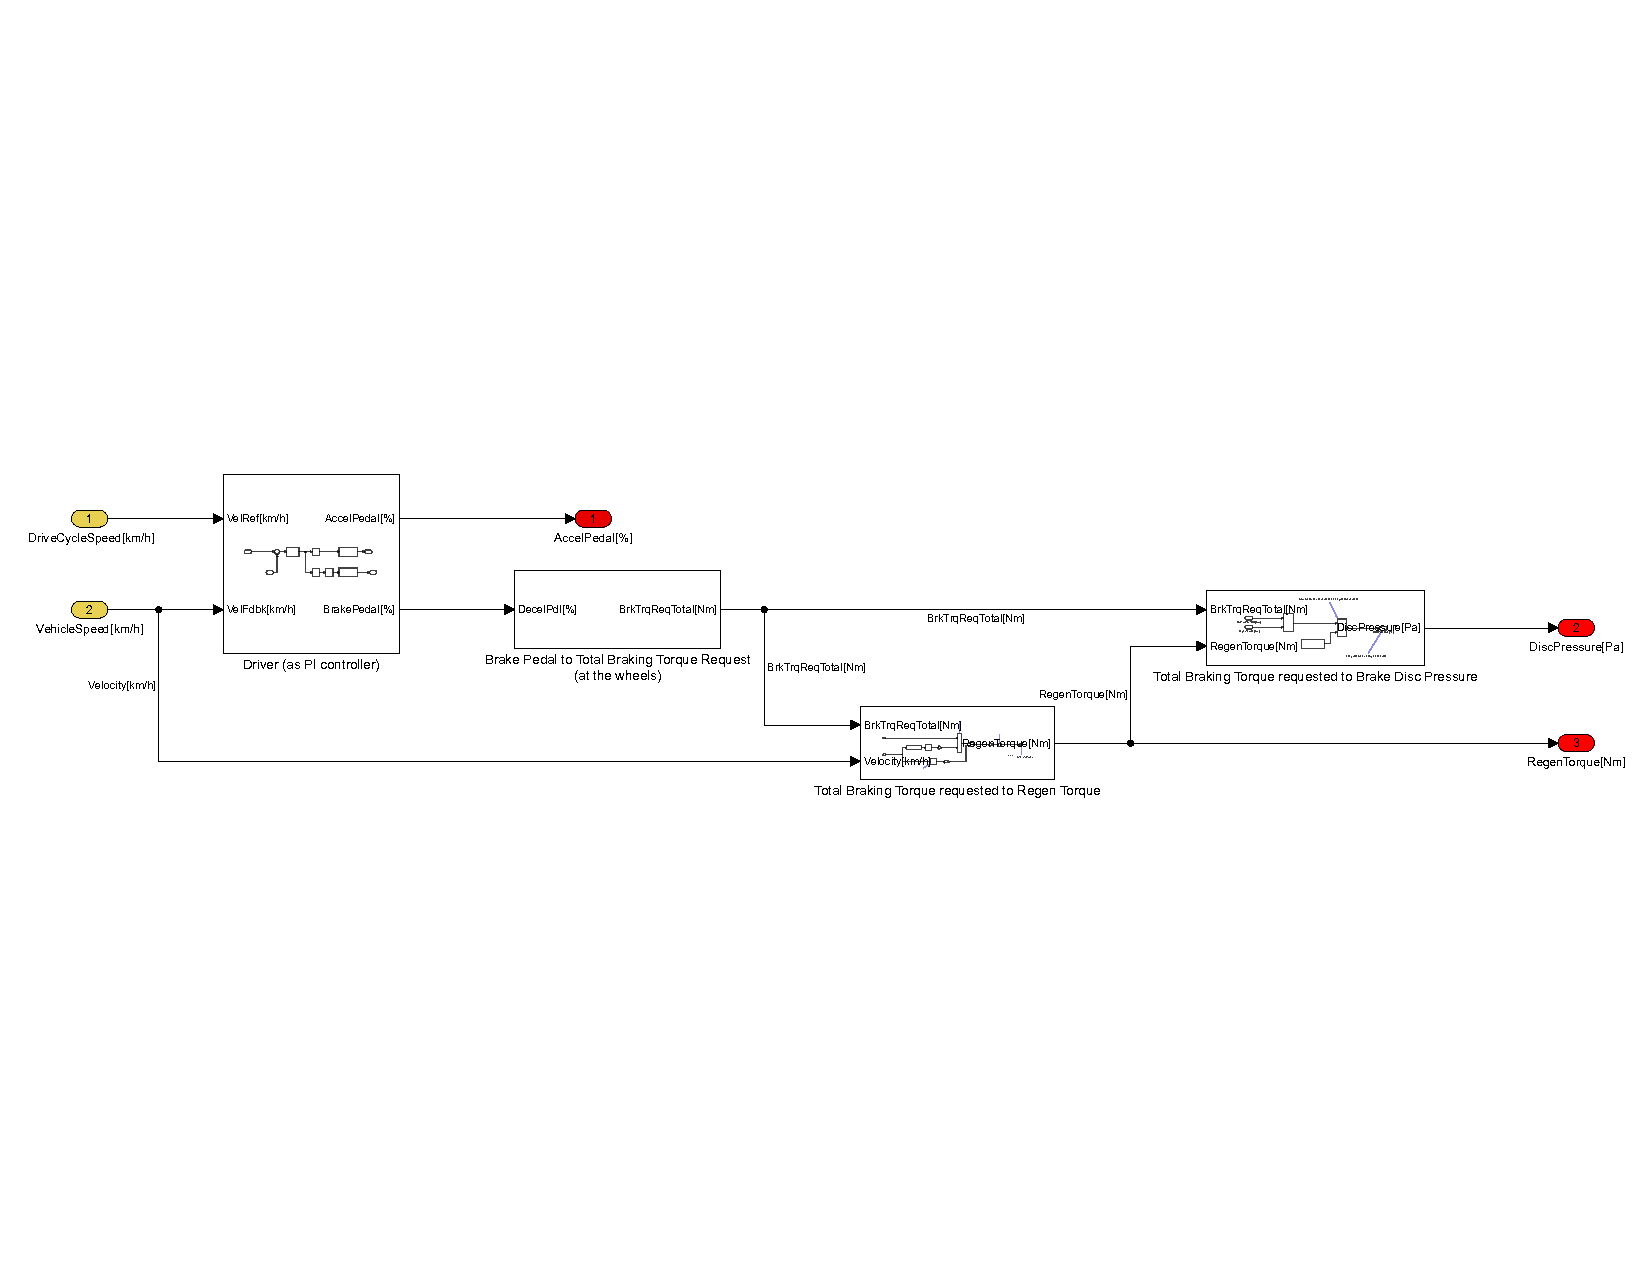
\includegraphics[width=\textwidth]{images/simulink_driver.pdf}
    \captionof{figure}{Simulink EV model - driver and braking subsystems}
    \label{fig:simulink_driver}
\end{minipage}
}

\newpage

\hspace{-1.5cm}
\rotatebox{90}{
\begin{minipage}{\textheight}
    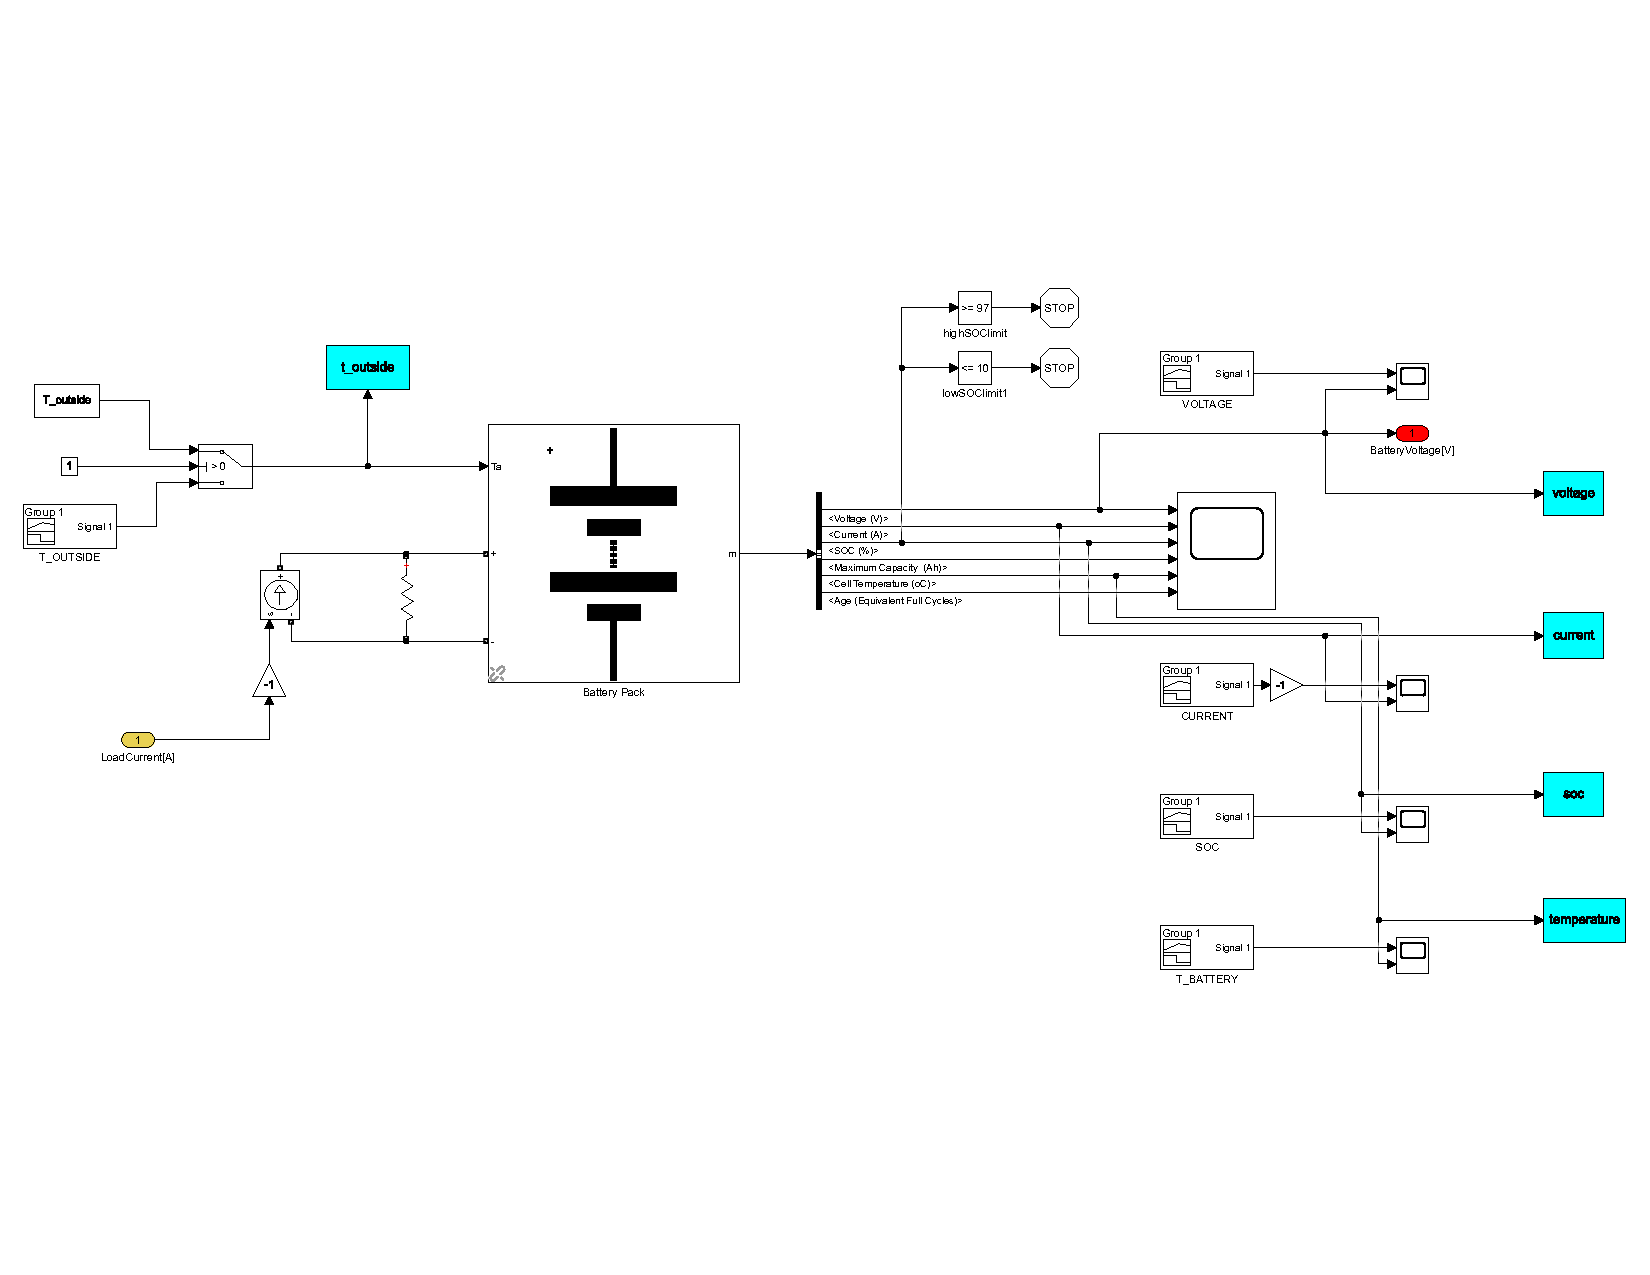
\includegraphics[width=\textwidth]{images/simulink_battery.pdf}
    \captionof{figure}{Simulink EV model - battery pack subsystem}
    \label{fig:simulink_battery}
\end{minipage}
}
\hspace{2cm}
\rotatebox{90}{
\begin{minipage}{\textheight}
    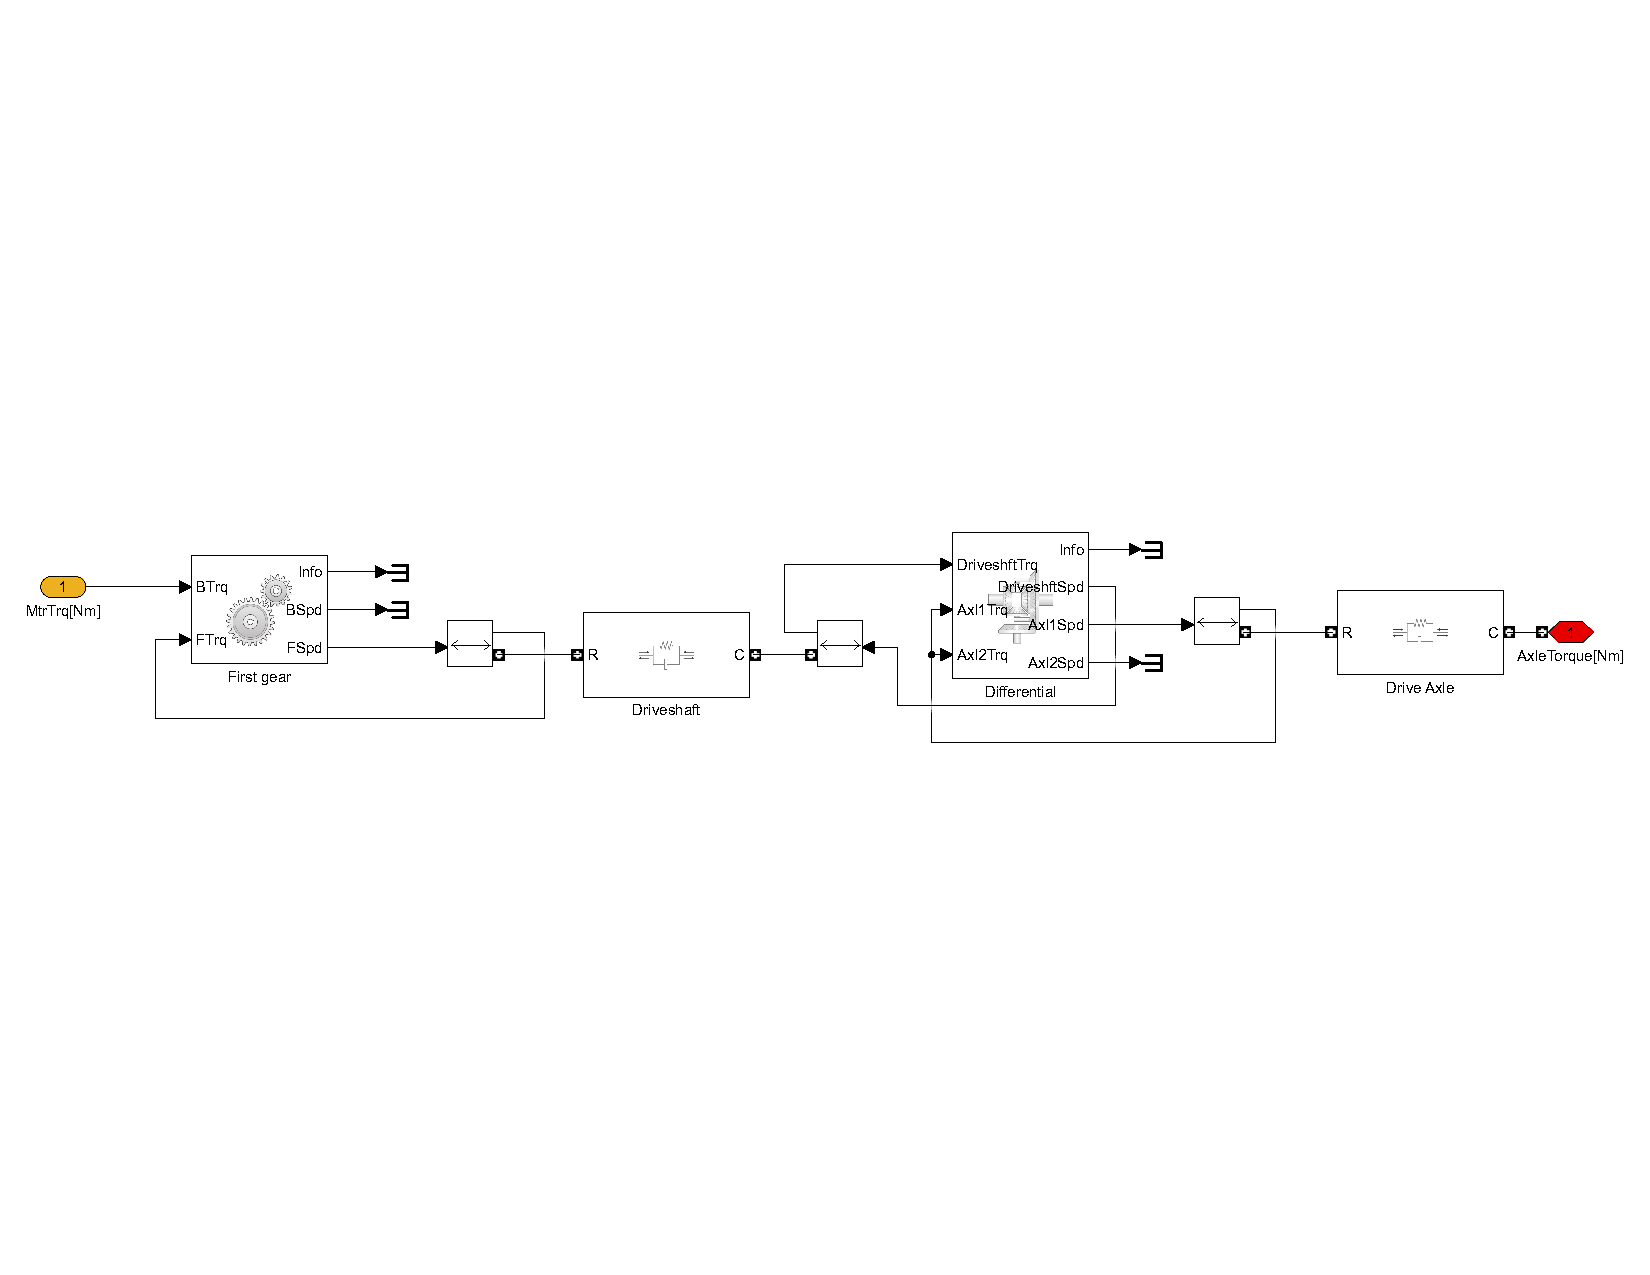
\includegraphics[width=\textwidth]{images/simulink_drivetrain.pdf}
    \captionof{figure}{Simulink EV model - drivetrain subsystem}
    \label{fig:simulink_drivetrain}
\end{minipage}
}

\newpage

\begin{figure}[H]
    \centering
    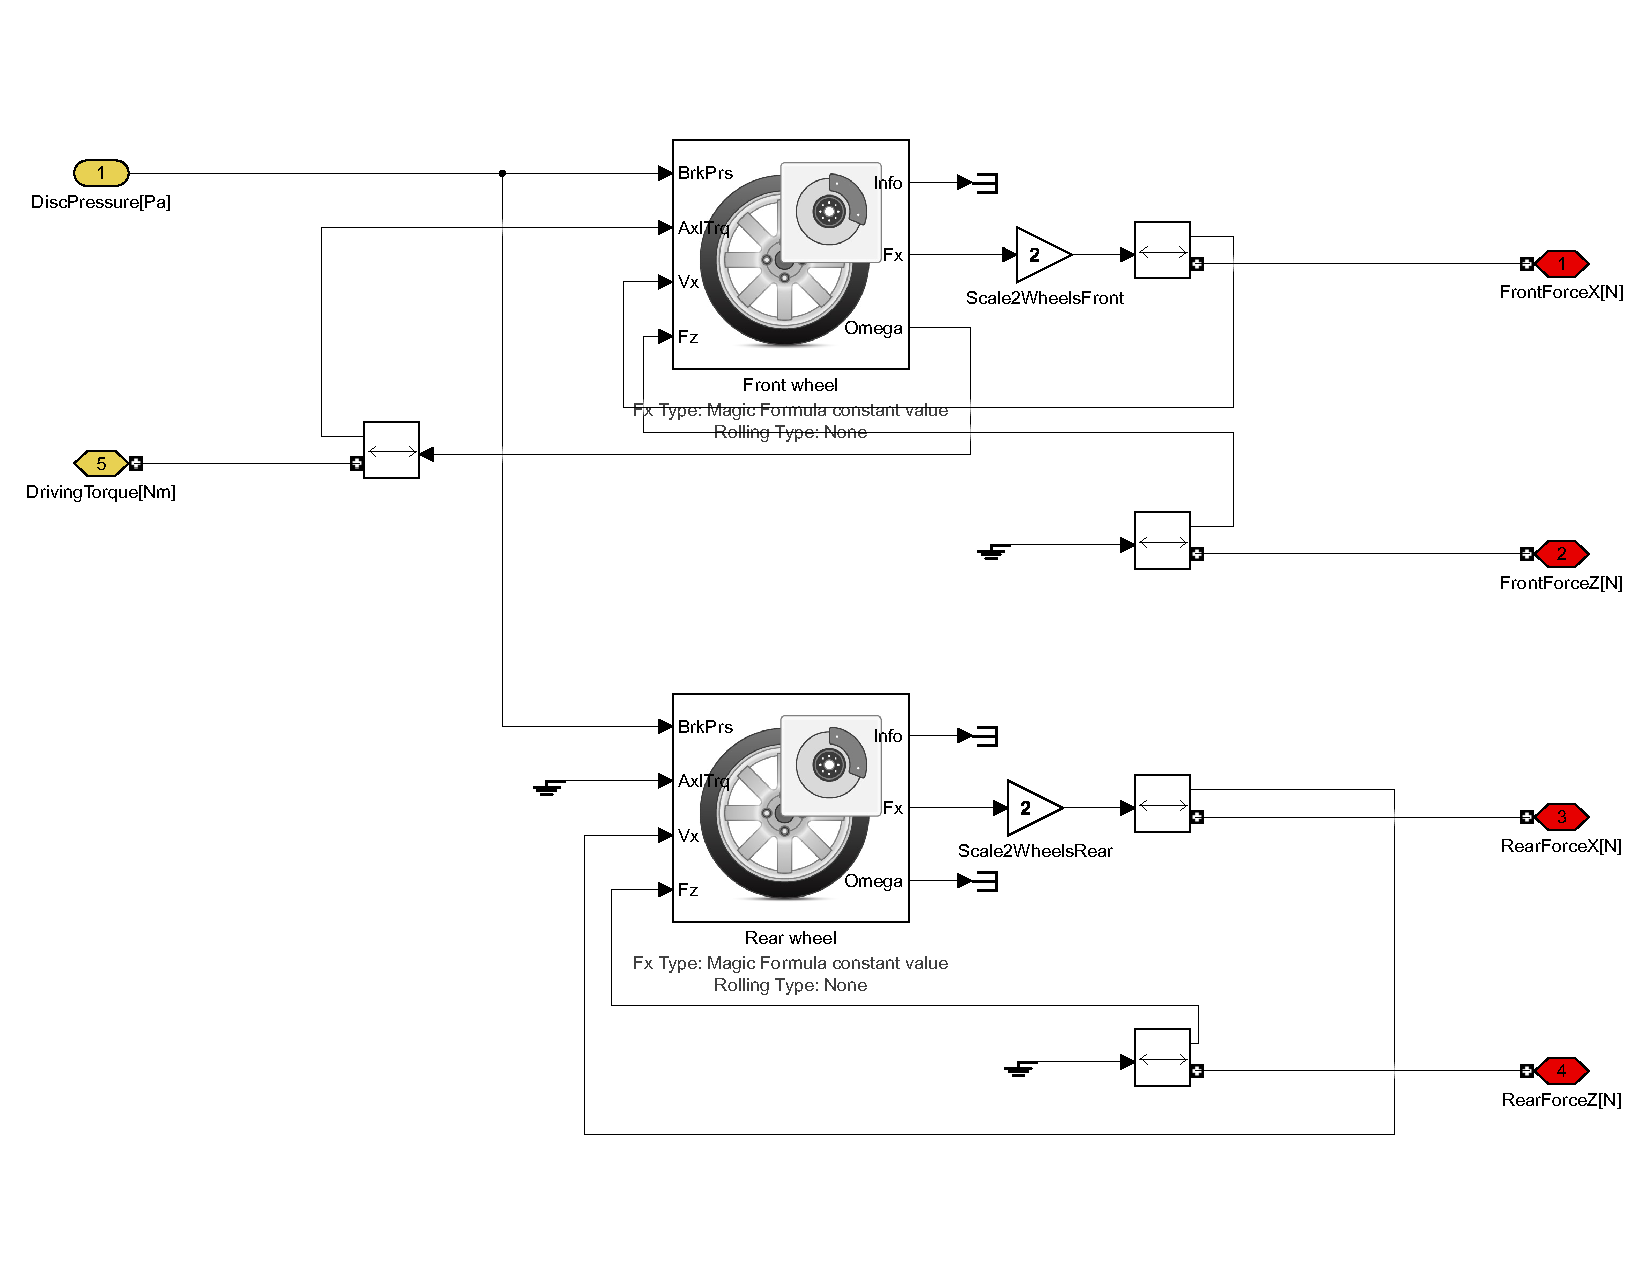
\includegraphics[width=0.95\textwidth]{images/simulink_wheels.pdf}
    \caption{Simulink EV model - wheels subsystem}
    \label{fig:simulink_wheels}
\end{figure}

\begin{figure}[H]
    \centering
    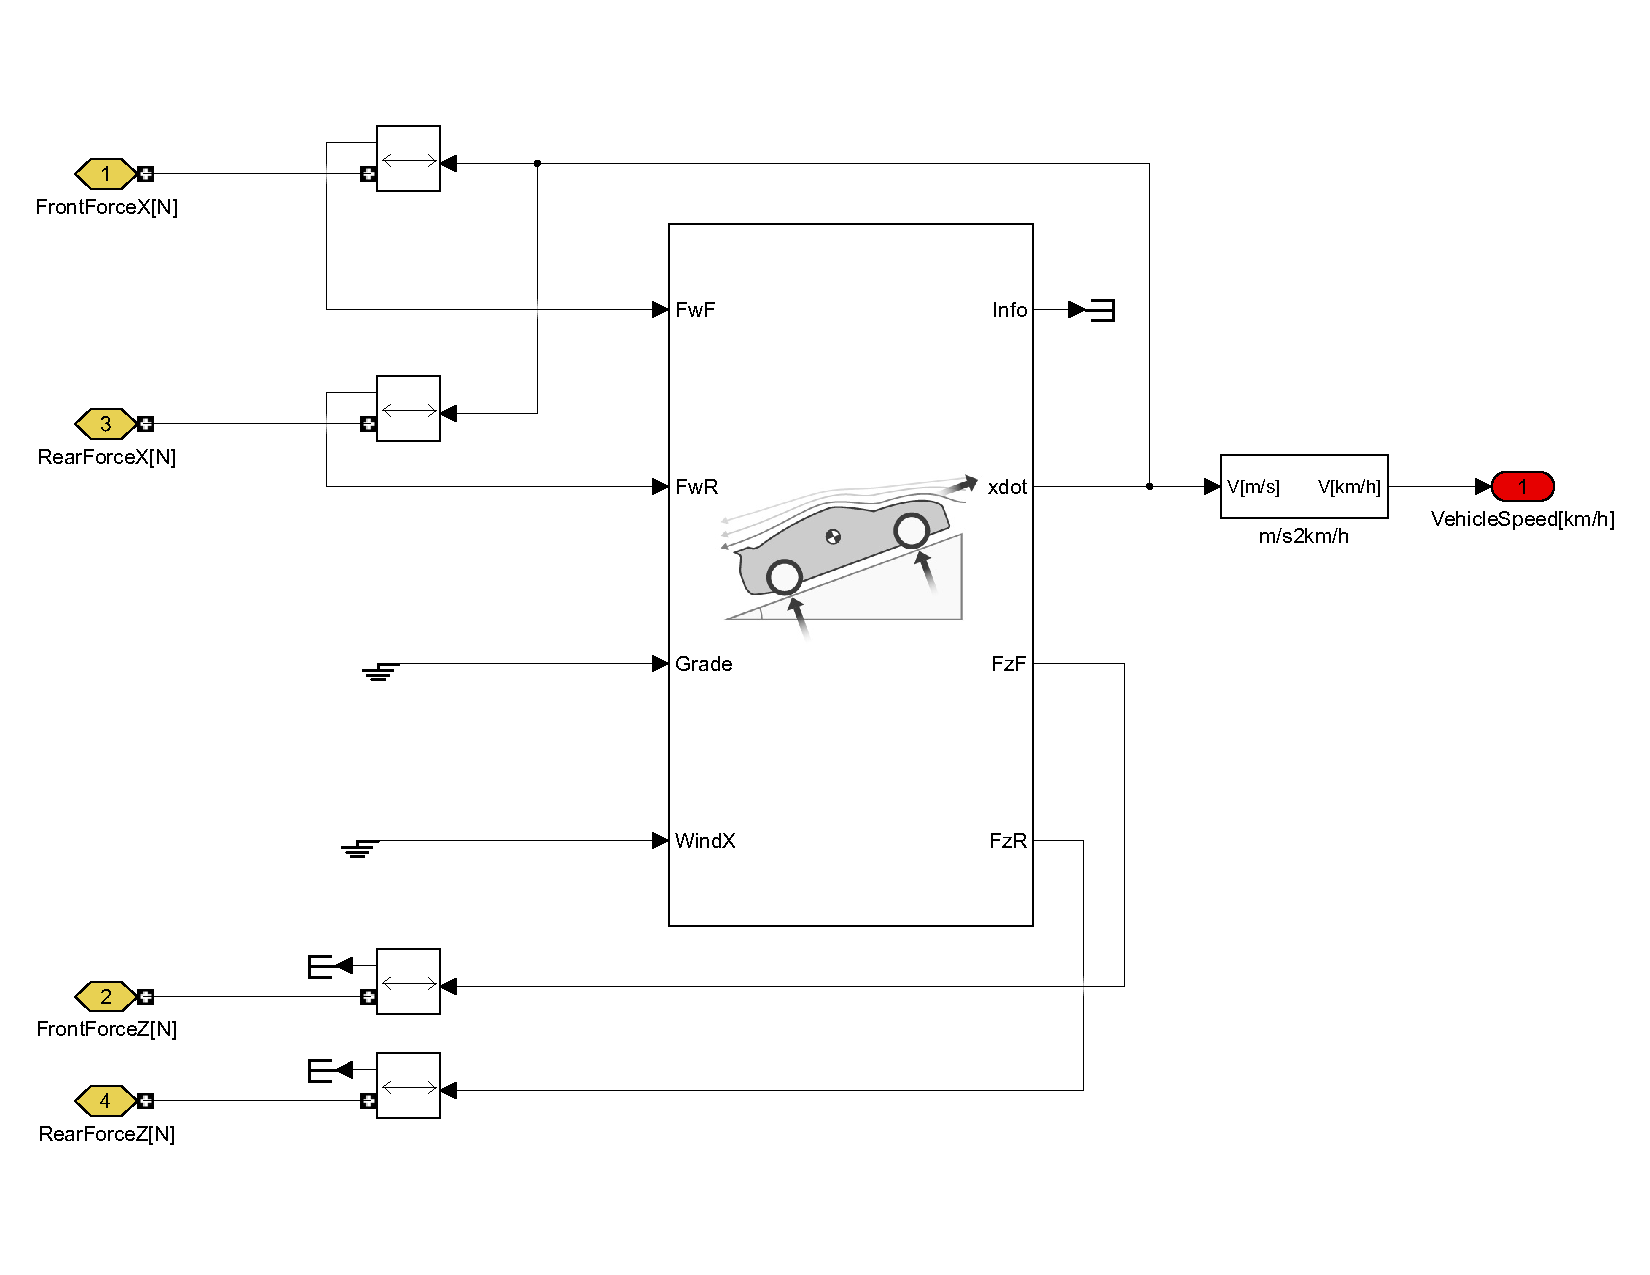
\includegraphics[width=0.95\textwidth]{images/simulink_body.pdf}
    \caption{Simulink EV model - vehicle body subsystem}
    \label{fig:simulink_body}
\end{figure}







\chapter{Additional notes}

\section{Spatial median}
\label{sec:spatial_median}
Spatial medians are a family of multivariate medians, i.e. an extension of the notion of univariate median to multivariate distributions. Multiple Theil-Sen estimation (sec. \ref{sec:theil-sen}) uses a particular spatial median defined via a depth function, first introduced in \cite{spatial_median}.

Let $\mathbf{Z} \in \mathbb{R}^d$ be a random vector with joint probability distribution $Q$. The statistical spatial depth is defined as
\[
D_\text{sp}(\mathbf{z},Q) = 1 - \norm{\mathbb{E}_Q S(\mathbf{z}-\mathbf{Z})}, \qquad \mathbf{z} \in \mathbb{R}^d
\]
where $S(\mathbf{v})=\mathbf{v}/\norm{\mathbf{v}}$ $(S(\mathbf{0})=\mathbf{0})$ is the spatial sign function, i.e. the projection of $\mathbf{v} \in \mathbb{R}^k$ to a $k$-sphere.

For a random sample $\mathbf{Z_1},\dots,\mathbf{Z_n}$ drawn according to $Q$, the sample spatial depth is defined as
\[
\Tilde{D}_\text{sp}(\mathbf{z},Q_n) = 1 - \norm{\frac{1}{n} \sum_{i=1}^n S(\mathbf{z}-\mathbf{Z_i})}, \qquad \mathbf{z} \in \mathbb{R}^d
\]
where $Q_n$ is the empirical distribution over the random sample. Then, the statistical (sample) spatial median $m$ ($\Tilde{m}$) is the maximizer of the statistical (sample) spatial depth, i.e.
\[
m = \argsup_{x\in\mathbb{R}^d} D_\text{sp}(\mathbf{x},Q) \qquad\qquad \Tilde{m} = \argsup_{x\in\mathbb{R}^d} \Tilde{D}_\text{sp}(\mathbf{z},Q_n)
\]

\newpage

\section{Time windows extraction}
\label{sec:tw_extr_alg}
The algorithm for extracting time windows from a dataset of driving sessions' data is the following

\begin{algorithm}
\caption{Time windows extraction}
\label{alg:time_window_extraction}
\begin{algorithmic}[1]
\State \# \textbf{Input arguments}
\State \texttt{dataset}: the dataset from which to extract time windows
\State \texttt{length}: duration of the time windows [s] (default: 300)
\State \texttt{slide}: time between the starting points of two consecutive time windows [s] (default: \texttt{length}, i.e. non-overlapping time windows)
\State \texttt{freq}: sampling rate of the measurements [Hz] (default: 5)
\State \texttt{max\_SOC}: time windows do not contain SOC values above this one (default: 100)
\State \texttt{min\_SOC}: time windows do not contain SOC values under this one (default: 0)
\State \texttt{random\_starting\_point}: choose the starting point of the first time window at random in the interval $[0,\text{\texttt{length}}]$ (default: true)
\State 
\State \# \textbf{Function}
\State \texttt{time\_windows\_dataset} $\gets$ empty list
\For{driving session $\in$ \texttt{dataset}}
\State \texttt{duration} $\gets$ duration of the current driving session
    \If{\texttt{random\_starting\_point}}
        \State \texttt{start} $\gets$ $\mathcal{U}(0,\text{\texttt{length}})$
    \Else
        \State \texttt{start} $\gets$ 0
    \EndIf
    \State \texttt{end} $\gets$ $\text{\texttt{start}} + \text{\texttt{length}}$
    \While{\texttt{end} $\leq$ \texttt{duration}}
        \State \texttt{time\_window} $\gets$ $[\text{\texttt{start}},\text{\texttt{end}}]$
        \If{SOC values in \texttt{time\_window} are between \texttt{max\_SOC} and \texttt{min\_SOC}}
            \State append data of \texttt{time\_window} to \texttt{time\_windows\_dataset}
        \EndIf
        \State \texttt{start} $\gets$ \texttt{start} $+$ \texttt{slide}
        \State \texttt{end} $\gets$ \texttt{end} $+$ \texttt{slide}
    \EndWhile
\EndFor
\State \textbf{return} \texttt{time\_windows\_dataset}
\end{algorithmic}
\end{algorithm}



\section{Hyperparameter tuning}
\label{sec:hyperparameter tuning}
The hyperparameters chosen for each regression model are reported in the following table.

\begin{table}[hbt!]
\footnotesize
\centering
\rotatebox{90}{
\begin{minipage}{0.88\textheight}
%\ra{1.3} % 30% more space between rows
\begin{tabular}{rccccccccccccccccc}
\toprule
& \multicolumn{3}{c}{Ridge} & \phantom{} & \multicolumn{2}{c}{Random forest} & \phantom{} & \multicolumn{6}{c}{Neural network}\\
\cmidrule{2-4} \cmidrule{6-7} \cmidrule{9-14}
& $\alpha$ & $\eta_0$ & $p$ && \breakcell{max. tree\\depth} & n. trees && \breakcell{neurons\\per layer} & \breakcell{max.\\epochs} & $\alpha$ & $\eta_0$ & $\mu$ & $P$\\
\midrule
\rule{0pt}{3ex}
\textbf{e-up!}\\
\cmidrule{1-1}
\textsc{MiniRocket} & 0.0278 & 0.001 & 0.25 && 30 & 1000 && $(120, 60, 40)$ & 300 & 0.0001 & 0.1 & 0.9 & 5\\
OLS & 0.01 & 0.0464 & 0.25 && 50 & 500 && $(40, 20)$ & 300 & 0.0001 & 0.1 & 0.9 & 5\\
Theil-Sen & 0.01 & 0.0464 & 0.25 && unlimited & 500 && $(40, 20)$ & 300 & 0.0001 & 0.1 & 0.9 & 5\\
\rule{0pt}{5ex}
\textbf{e-Golf}\\
\cmidrule{1-1}
\textsc{MiniRocket} & 0.01 & 0.0008 & 0.25 && 30 & 1000 && $(120, 60, 40)$ & 300 & 0.0001 & 0.1 & 0.9 & 5\\
OLS & 0.01 & 0.0464 & 0.25 && 15 & 500 && $(40, 20)$ & 300 & 0.0001 & 0.1 & 0.9 & 5\\
Theil-Sen & 0.01 & 0.0464 & 0.25 && 15 & 500 && $(40, 20)$ & 300 & 0.0001 & 0.1 & 0.9 & 5\\
\bottomrule
\end{tabular}
\caption[Chosen hyperparameters]{Hyperparameters chosen for each regression model and training set. $\alpha$ is the regularization factor, $\eta_0$ is the initial learning rate. The ridge regression model is trained via SGD with learning rate computed at each iteration as $\eta(i) = \eta_0 / i^p$. The neural network is trained via SGD with learning rate divided by 10 whenever the training loss doesn't decrease enough for $P$ consecutive epochs.}
\end{minipage}}
\label{tab:hyperparameters}
\end{table}